\chapter{Methodology}
\label{chap:methodology}
In this section a performance model for understanding the runtime characteristics of deep learning models is outlined. To understand these characteristics, the underlying factors that affect it need to be understood first. 


\section{Problem Space}
The inference performance of a deep learning model is mainly affected by two major parts, the structure of the model itself and the hardware environment where it gets deployed. A third factor is the serving framework.

\subsection{Deployment}
Model deployment describes the process of deploying a trained machine learning model to a production environment for inference purposes. 

There can be differentiated in two different deployment methods, the first one is deploying the model directly to edge devices, while the second outsources the model to a cloud-backend, where the inference is performed and the prediction is sent back to the edge device.
\subsubsection{Edge Deployment}
Edge devices are characterized by offering a limited amount of hardware and are often mobile, which results in a limited amount of available energy, memory and overall computational power.
Example devices are smartphones, cars or Raspberry Pis.
Despite its limits, edge deployment also has some advantages, particular in reliability and security. 
For example in the case of image classification images are needed for the inference, which often contain sensible information and thus raise a data privacy/security concern.
Therefore edge deployment is preferred, if the inference performance is sufficient.

In order to increase this performance various accelerators like better GPUs, TPUS or other dedicated neural network hardware components have been developed for edge devices.

\begin{itemize}
    \item Was ist Edge (Beispiele)
    \item Was macht Edge aus?
\end{itemize}
\subsubsection{Cloud Deployment}
While the breakthroughs in deep learning is very interesting for AI applications on the edge devices, the computational demand needed for edge deployment often exceeds the available power to be viable.
That is why the option of outsourcing the models to a cloud-backend has become a popular solution in the recent years.
Cloud-backend offer a huge amount of computational power, especially suitable for deep learning in the form of GPUs, TPUs, etc.


The big downside of cloud-based inference is the needed network connection, in particular for edge devices such as cars, where a reliable network connection can often not be guaranteed for example in rural areas. Hence this is not a viable solution for applications that are critical like autonomous driving.
\begin{itemize}
    \item Was ist cloud?
    \item Was macht cloud aus
\end{itemize}

\subsection{Deep Learning}
Deep learning models are defined as neural networks with many layers and hidden units, the most popular being convolutional neural networks and recurrent neural networks right now, which are special forms of neural networks.
There are many different operators, which makes performance prediction very complex.
In the following the two most popular networks get analyzed.
%This increased amount of layers leads to complex mathematical calculations.
\subsubsection{Quantization}
Quantization is a technique that trades in model precision for better inference times, memory consumption during inference and model sizes.
Quantization describes the process of reducing the "precision representations of weights and, optionally, activations" \cite{tfLiteQuant} from floating point precision to for example 8-bit.
The weights/activations are either quantized after training the model with floats (Post Training Quantization) or the model is training with quantized weights/activations from the start (Quantization Aware Training). In the paper "Quantizing deep convolutional networks for
efficient inference"\cite{Quantizing} Krishnamoorthi performed a study on these technique with the following results:
8-bit quantization can lead to a model size reduction by a factor of 4, a 2x-3x latency speedup on CPUs and DSP, while reducing the model accuracies by 1\%

\begin{itemize}
    \item layer
    \item hidden units
    \item input size
    \item number of operations
\end{itemize}
\subsubsection{Convolutional Neural Network}
This special subclass of neural network achieved wide success in the field of object recognition and detection in images. Convolutional Neural Networks (CNN)
\paragraph{Input}
The input of CNNs often consists of images, but also can be...

\paragraph{Operations}
filter, pool, 
\subsubsection{Recurrent Neural Network}
%%%WIRKLICH MACHEN ODER NUR CNNs?
Recurrent neural networks (RNN) are made for the processing of sequences and made a lot a progress in the fields of voice recognition.
\paragraph{Input}
seqeuences
\paragraph{Operations}
GRU, LTSM
\begin{itemize}
    \item parameter von Modellen
    \item Was für Einfluss haben diese Parameter?
\end{itemize}


\section{Performance Model}
All the aspects of both hardware and model have an impact on the performance, thus are the inputs of the performance model (see figure \ref{fig:perfmodel}). These inputs affect various performance metrics, of which inference time and throughput are the most important ones for real-time AI applications. However, as the hardware on edge devices is limited and most of the times many applications need to run in parallel, low usages of the other metrics are vital as well.
While accuracy is one of the most critical metrics for computer vision networks, it is only affected by the characteristics of the model and not by the deployment environment. Therefore we do not focus on accuracy in this thesis.
To get the model output for a given model input two steps are needed. The first one is the preprocessing step and transforms a given input into the format that is required by the deep learning model. Only then the actual inference operation can be performed to obtain the model output. Therefore the preprocessing takes a vital part in the general inference process and should be included in the performance model.
\begin{figure}[H]
\centering
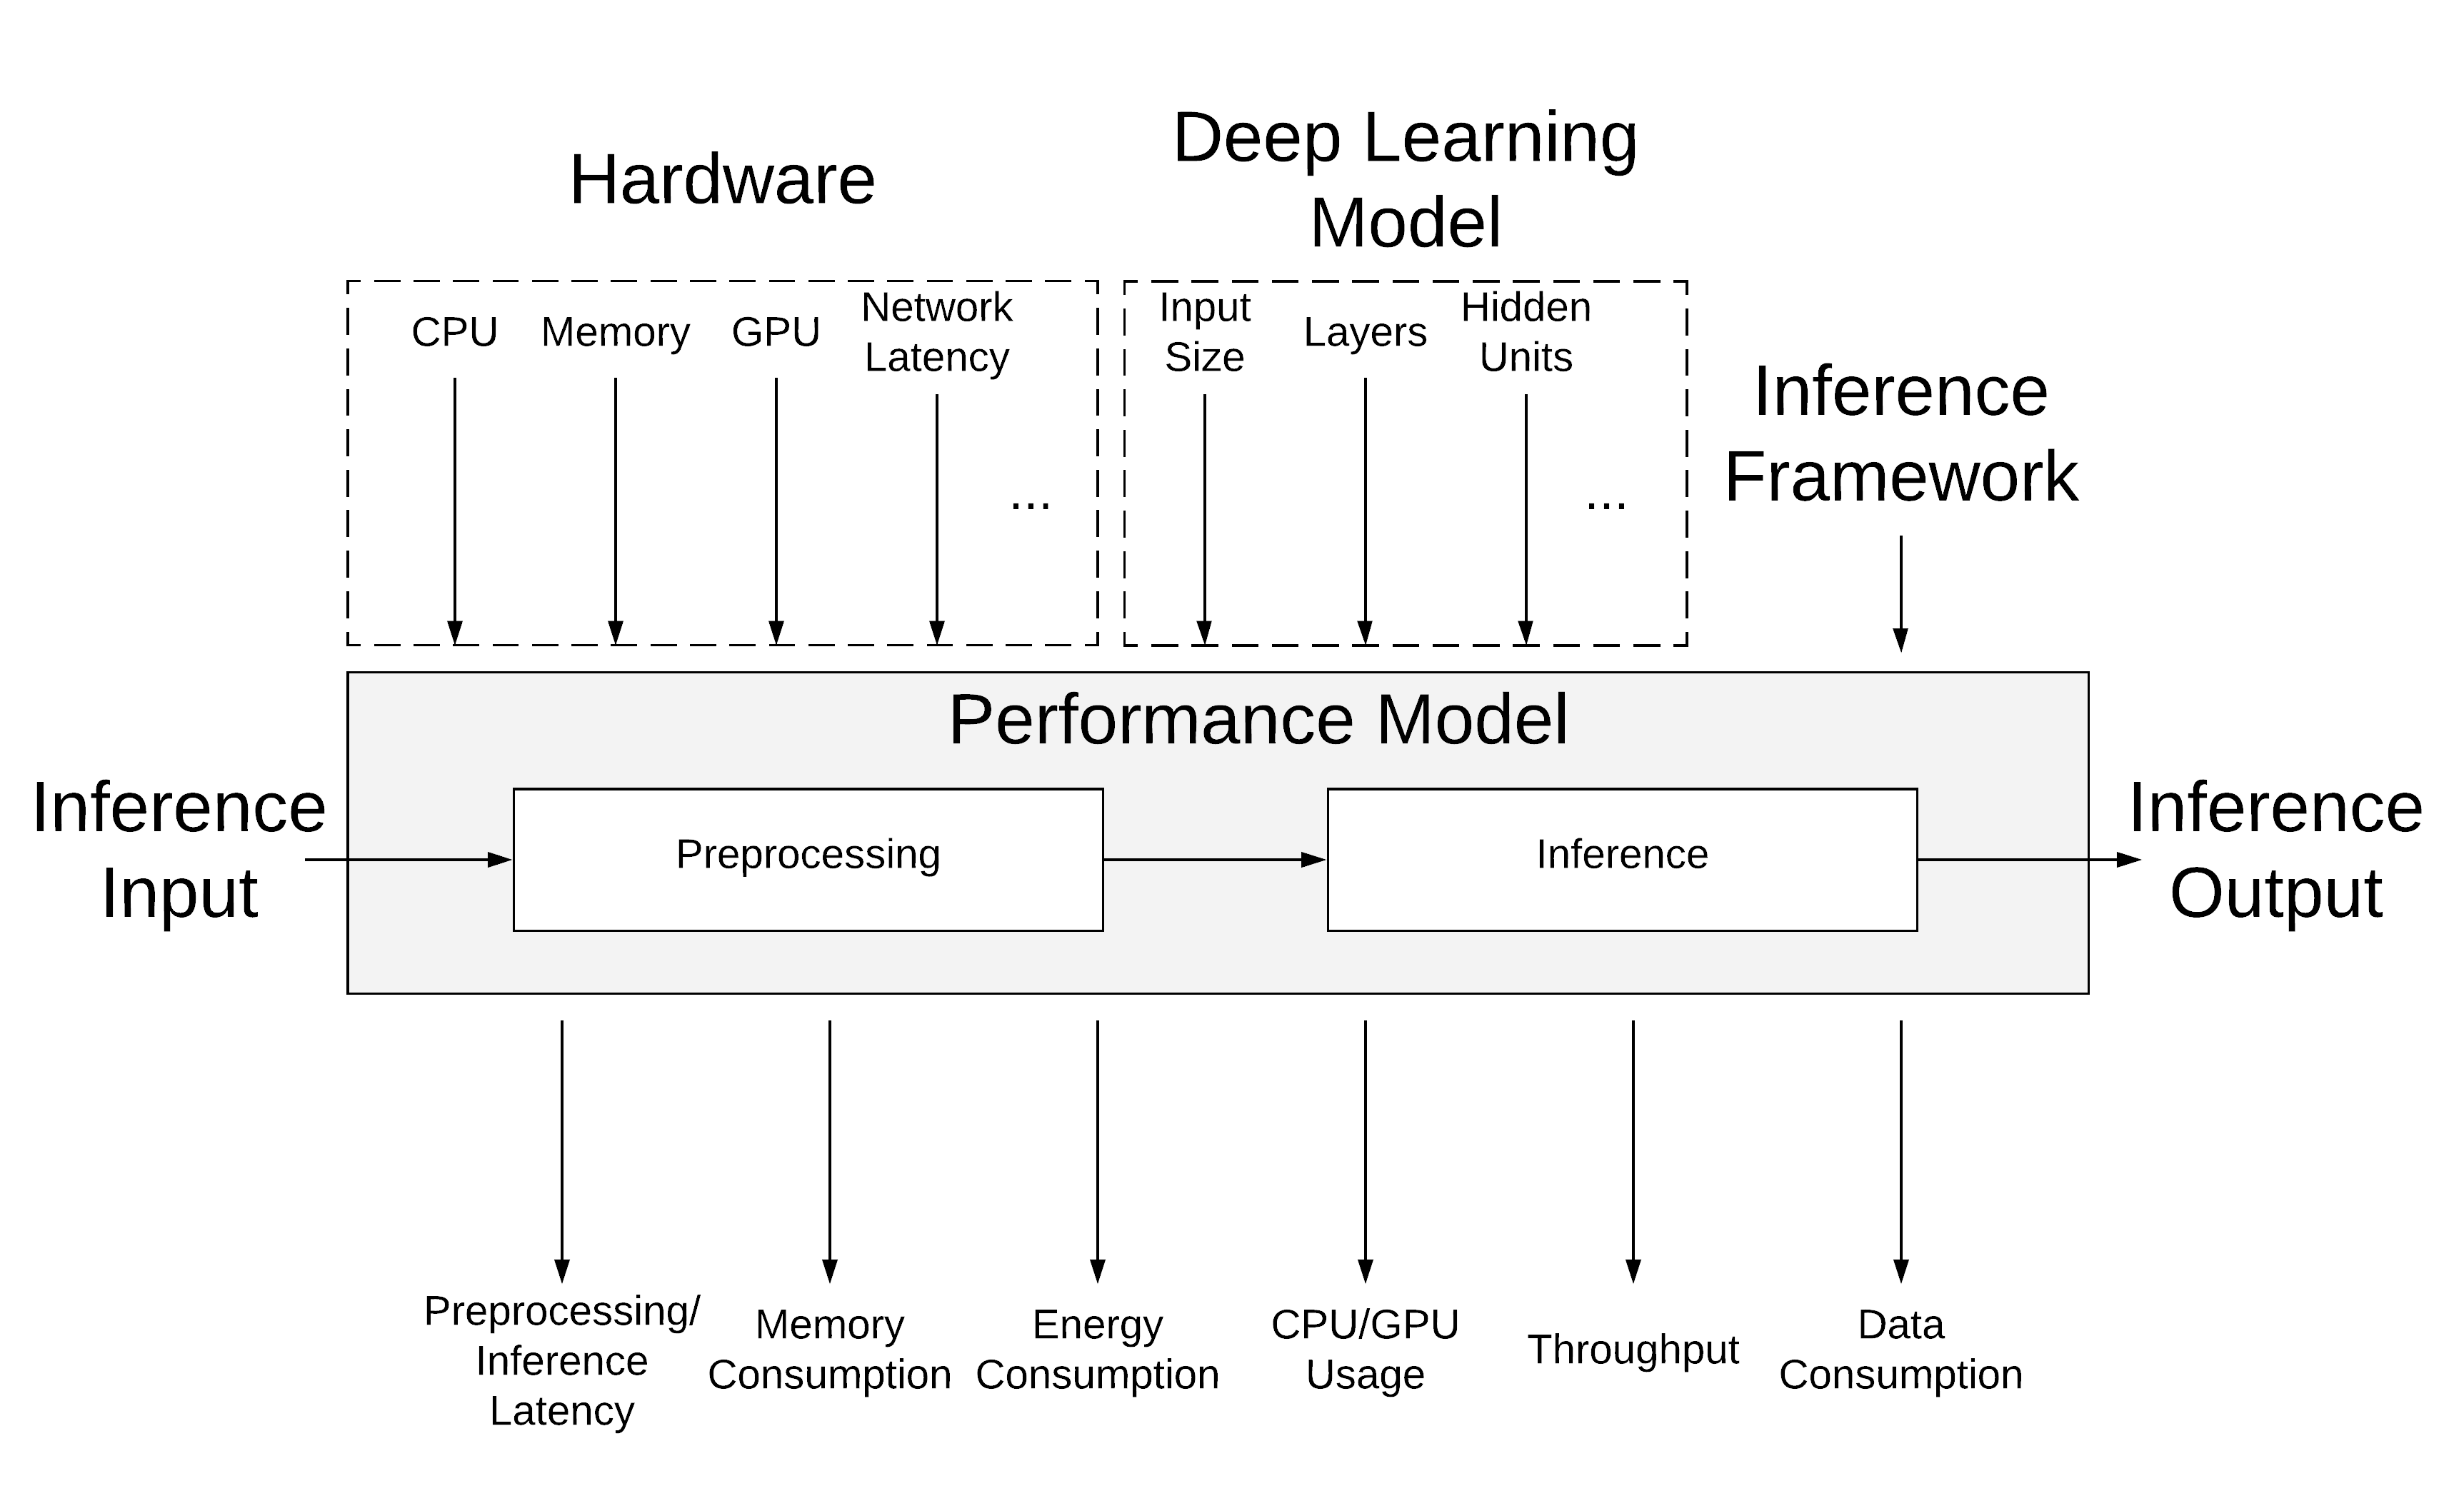
\includegraphics[width=0.99\textwidth]{./Bilder/trade_offs.png}
\caption{Performance Model}
\label{fig:perfmodel}
\end{figure}
\subsection{Performance Metrics}
Several metrics are important to measure the performance of the preprocessing and the inference steps. 
 
\subsubsection{Inference Time}
%%WALL CLOCK TIME ADD HERE
Inference time describes the time needed from requesting a prediction from a deep learning model given an specific input until getting the prediction.
This metrics is essential for the performance, since AI application often need predictions in realtime.
\subsubsection{Preprocessing Time}
The time needed to transform the original input to a shape fit for feeding into the deep learning model is called preprocessing time.
\subsubsection{Energy Consumption}
This metric is particular important for mobile edge devices, since they often are powered by batteries with a limited lifespan. So if the inference process of a model consumes too much energy, the application using the model is not viable.
\subsubsection{CPU Usage}
Since the inference operation is most of the time not the only process running on a system and other processes need to run simultaneously to the inference, the CPU usage is an important metric.
\subsubsection{Memory Usage}
Similar to CPU usage, inference should not occupy the whole memory of system or even demand more memory than the available memory of a edge devices.
\subsubsection{GPU Usage}
If a GPU or an another accelerator is available their usage is of interest.
\subsubsection{Throughput}
In order to accomplish realtime AI a high enough throughput is essential. Therefore the number of processed predictions per second is a valuable metric. This metric can,depending on the specification, either mean preprocessing and inference together or only one of the two.
\subsubsection{Data Consumption}
This metric is only relevant for cloud inference as the request has to be sent to the cloud-backend and the according response with prediction has to be sent back to the client. A high data consumption could slow down the inference time significantly if the up- and downstream of the network connection is too slow. 

\endinput 